
\chapter{SWITCH 方式のしきい値の評価}
\label{sec:appendix1}

\refsec{eval_threshold}で説明したしきい値に関する評価に関して,既に説明した(8,2)以外のセグメント数の組み合わせでの評価結果を示す.評価手順は\refsec{eval_threshold}で説明したものと同様である.なお,ILP の評価値としては ISR と IPC よりも有効であることから,ISR のしきい値の評価に関しては省略し,IPC と LLC MPKI のしきい値の評価のみ説明する.

評価結果を,\fig{4_1_IPC}から\fig{8_4_MPKI}に示す.各図は,IPC 及び  LLC MPKI を変化させた場合の,SWITCH 方式において CONSERVATIVE モードで実行される割合を示している(\fig{switch_IPC_rate}や\fig{switch_MPKI_rate}と同様の形式).

これらの評価をもとに,(8,2)の場合と同様に最適なしきい値を求めた.各セグメント数での最適と判断したしきい値を\tab{switch_threshold_all}に示す.

LLC MPKI に関しては,全ての組み合わせにおいて 2.0 と同一のしきい値となっている.これは,セグメント数が変化しても,LLC MPKI はほとんど変化しないためである.

これに対して, IPC のしきい値はセグメントの総数が 16 までは共通で 3.5 となっているが,セグメントの総数が 32 の組み合わせにおいては,3.0 や 2.5 と最適なしきい値が低下していることがわかる.この理由を説明する.

ILP のしきい値が変化している理由は,cactusBSSN ベンチマークにおいてセグメントの総数が 32 の場合に急激に性能が低下するためである.cactusBSSN は ILP の高いベンチマークの一つで,BASE モデルにおいて IPC が 3.6 程度である.セグメントの総数が 16 以下の場合,このベンチマークは AGGRESSIVE モードにおいても大きな性能低下を起こさないが,セグメントの総数が 32 の場合にはAGGRESSIVE モードで 10\% 以上の大きな性能低下を起こす.その際,IPC は 3.3 程度((16,2)の場合)となる.

この場合に,IPC のしきい値が 3.5 であるような例を考える.このとき,AGGRESSIVE モードでの IPC は 3.3 であるためしきい値を下回り,ILP が低いと判定される.その結果,本来 ILP が高いと評価され CONSERVATIVE モードで実行されるべきであるが,AGGRESSIVE モードで実行され,性能が低下する.実際に,IPC のしきい値が 3.5 の場合には,\fig{16_2_IPC}の cactusBSSN を見るとわかるように CONSERVATIVE モードの割合が低いことがわかる.

このように,セグメントの総数が多い場合には,IPC のしきい値が高い場合に,本来 ILP が高いと判定したいプログラムにおいて,AGGRESSIVE モードでの性能低下が大きく,その結果 ILP が低いと誤って判定されることがある.したがって,セグメントの総数を多くする場合には,IPC のしきい値をある程度低く設定し,ILP の誤った判定を防ぐ必要があると言える.

\begin{table}[tb]
  \caption{セグメント数ごとの SWITCH 方式のしきい値}
  \footnotesize
  \center
    \begin{tabular}{c|c|c|c} \hline \hline
    総セグメント数 & (M-seg,S-seg) & IPC & LLC MPKI \\ \hline
    4 &(4,1) & 3.5 & 2.0 \\
    &(2,2) & 3.5 & 2.0 \\ \hline
    8 &(8,1) & 3.5 & 2.0 \\
    &(4,2) & 3.5 & 2.0 \\ \hline
    &(16,1) & 3.5 & 2.0 \\
    16 &(8,2) & 3.5 & 2.0 \\
    &(4,4) & 3.5 & 2.0 \\ \hline
    &(32,1) & 2.5 & 2.0 \\
    32 &(16,2) & 3.0 & 2.0 \\
    &(8,4) & 3.0 & 2.0 \\ \hline
  \end{tabular}
  \label{tab:switch_threshold_all}
\end{table}

%(4,1)
\begin{figure}[tb]
  \centering
  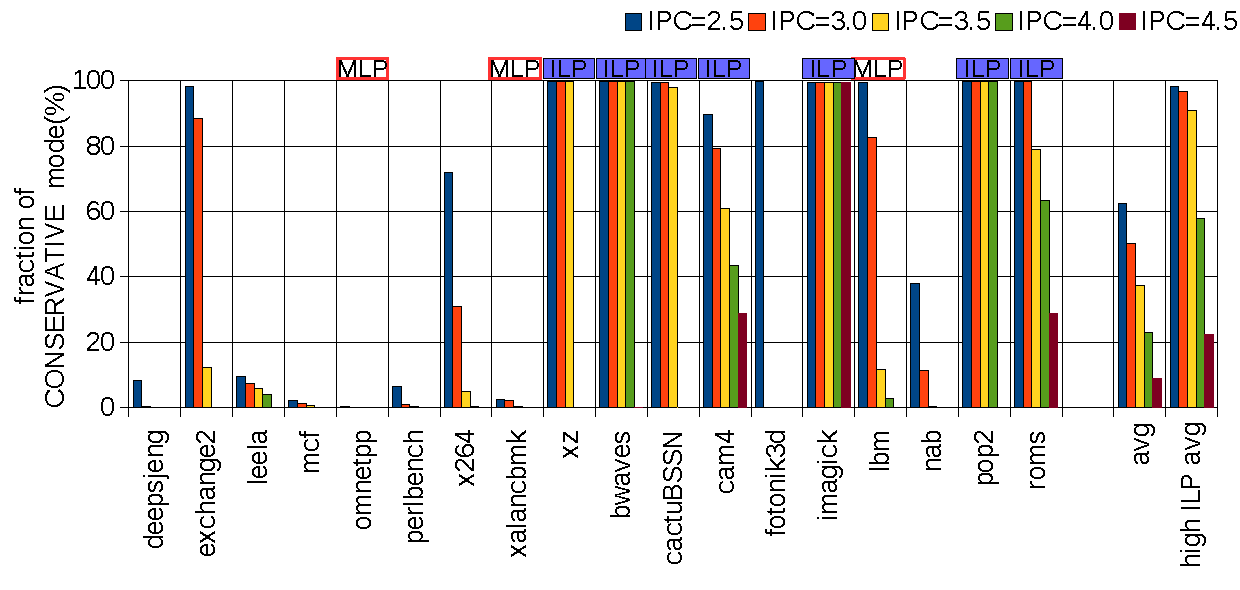
\includegraphics[keepaspectratio, scale=.8]{4_1_IPC}
  \caption{IPC を用いた SWITCH 方式の制御(4,1)}
  \label{fig:4_1_IPC}

  \centering
  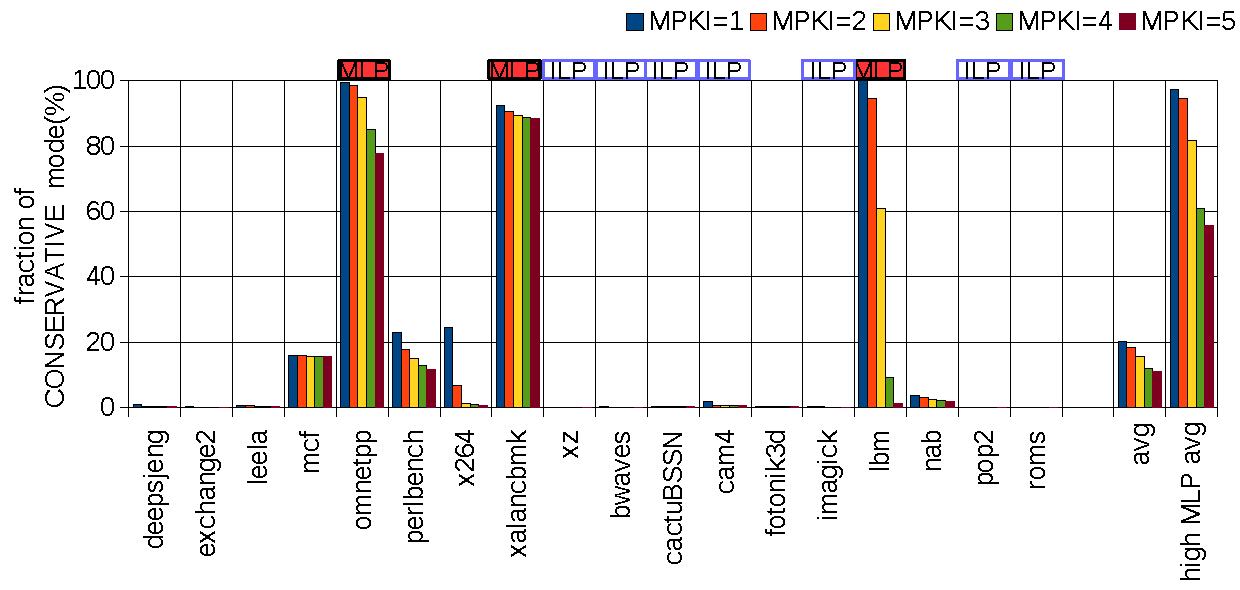
\includegraphics[keepaspectratio, scale=.8]{4_1_MPKI}
  \caption{LLC MPKI を用いた SWITCH 方式の制御(4,1)}
  \label{fig:4_1_MPKI}
\end{figure}

%(2,2)
\begin{figure}[tb]
  \centering
  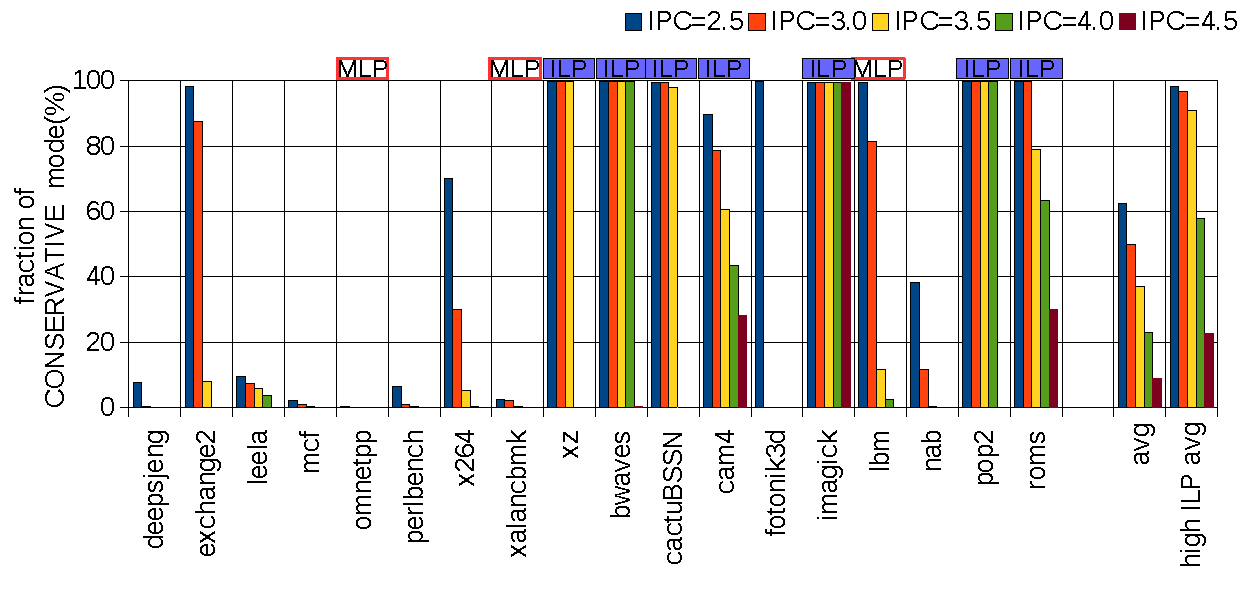
\includegraphics[keepaspectratio, scale=.8]{2_2_IPC}
  \caption{IPC を用いた SWITCH 方式の制御(2,2)}
  \label{fig:2_2_IPC}

  \centering
  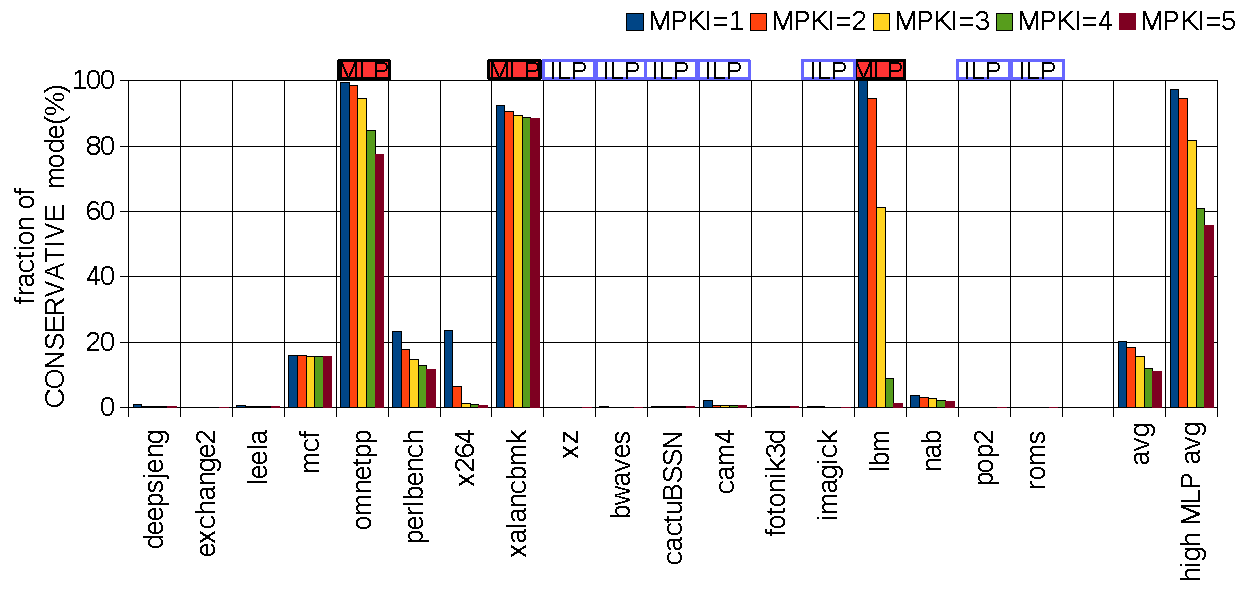
\includegraphics[keepaspectratio, scale=.8]{2_2_MPKI}
  \caption{LLC MPKI を用いた SWITCH 方式の制御(2,2)}
  \label{fig:2_2_MPKI}
\end{figure}

%(8,1)
\begin{figure}[tb]
  \centering
  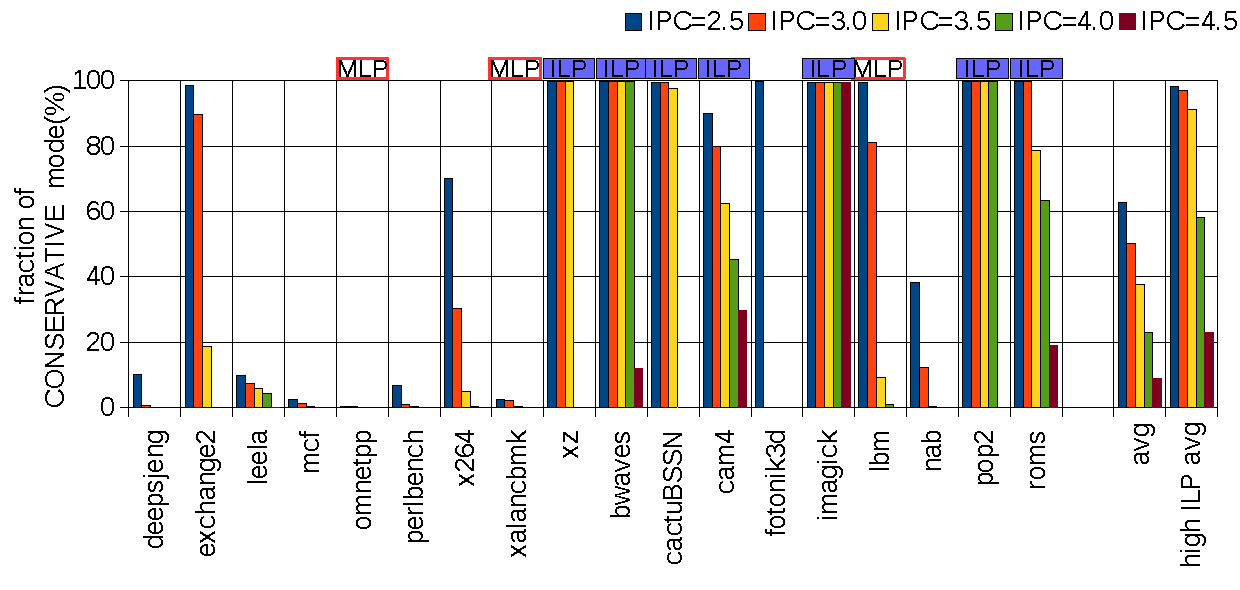
\includegraphics[keepaspectratio, scale=.8]{8_1_IPC}
  \caption{IPC を用いた SWITCH 方式の制御(8,1)}
  \label{fig:8_1_IPC}

  \centering
  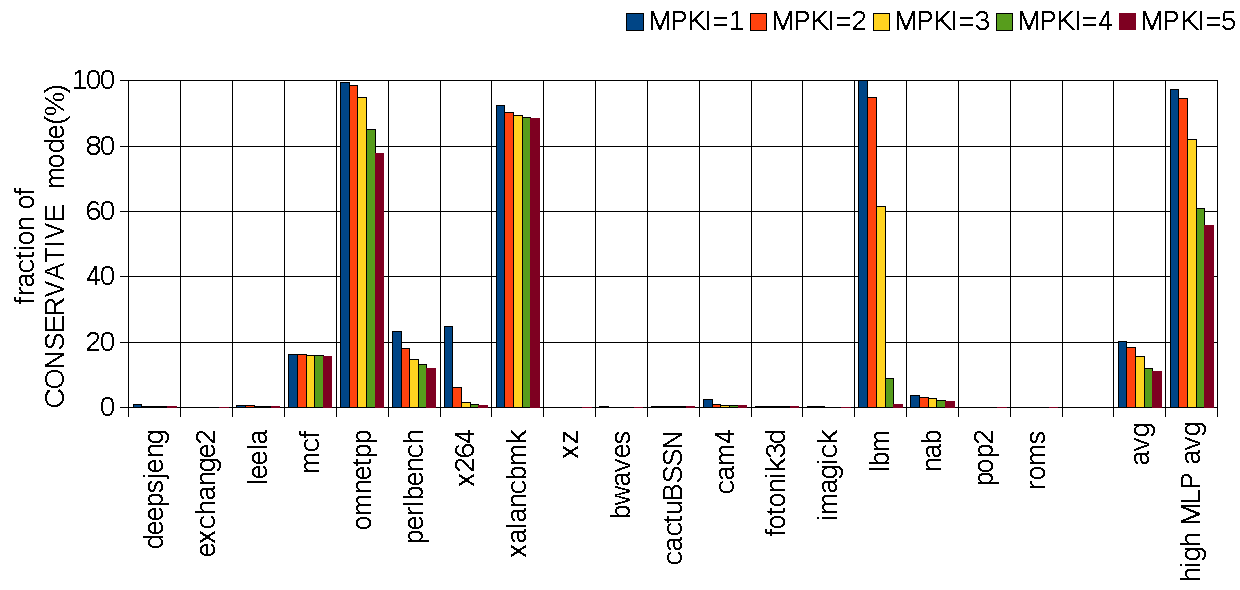
\includegraphics[keepaspectratio, scale=.8]{8_1_MPKI}
  \caption{LLC MPKI を用いた SWITCH 方式の制御(8,1)}
  \label{fig:8_1_MPKI}
\end{figure}

%(4,2)
\begin{figure}[tb]
  \centering
  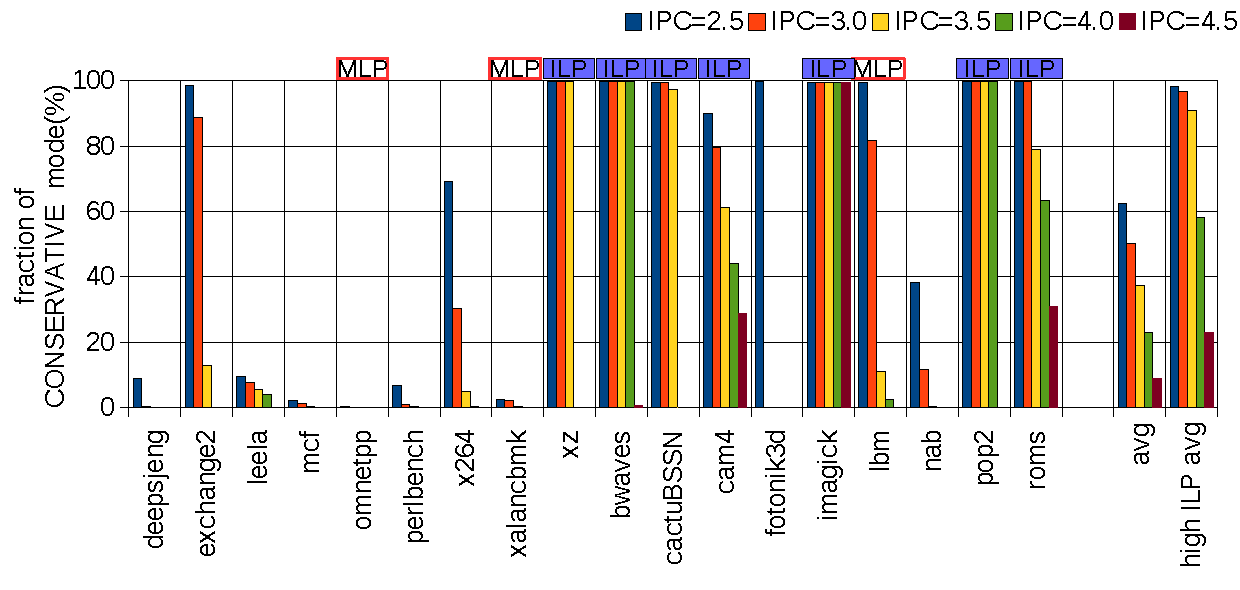
\includegraphics[keepaspectratio, scale=.8]{4_2_IPC}
  \caption{IPC を用いた SWITCH 方式の制御(4,2)}
  \label{fig:4_2_IPC}

  \centering
  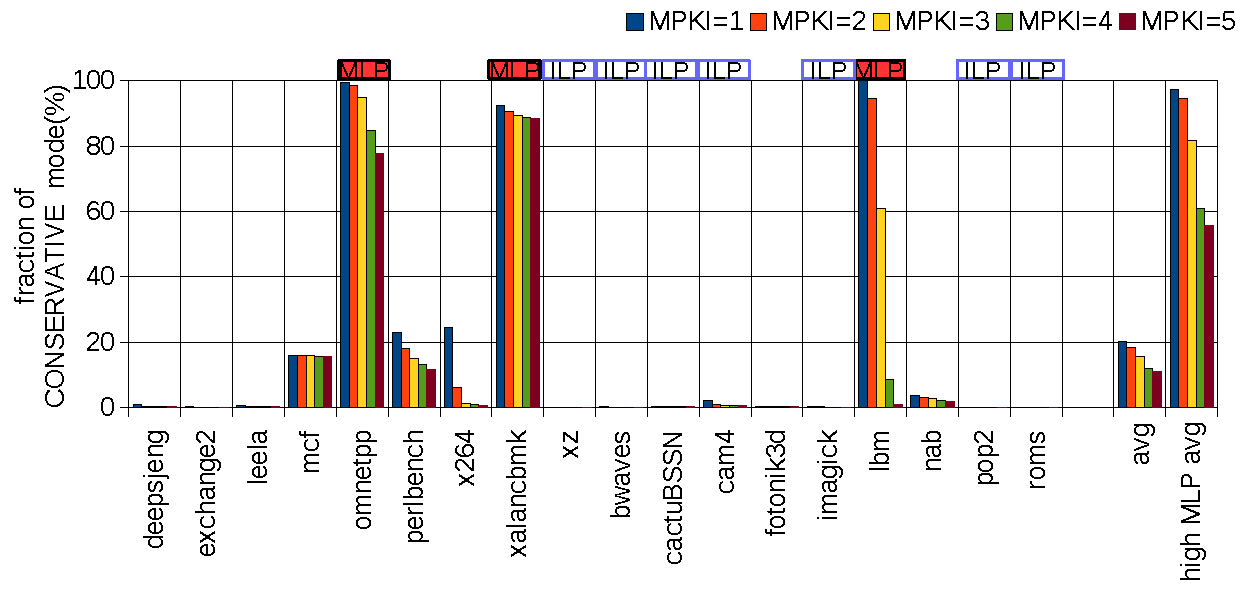
\includegraphics[keepaspectratio, scale=.8]{4_2_MPKI}
  \caption{LLC MPKI を用いた SWITCH 方式の制御(4,2)}
  \label{fig:4_2_MPKI}
\end{figure}

%(16,1)
\begin{figure}[tb]
  \centering
  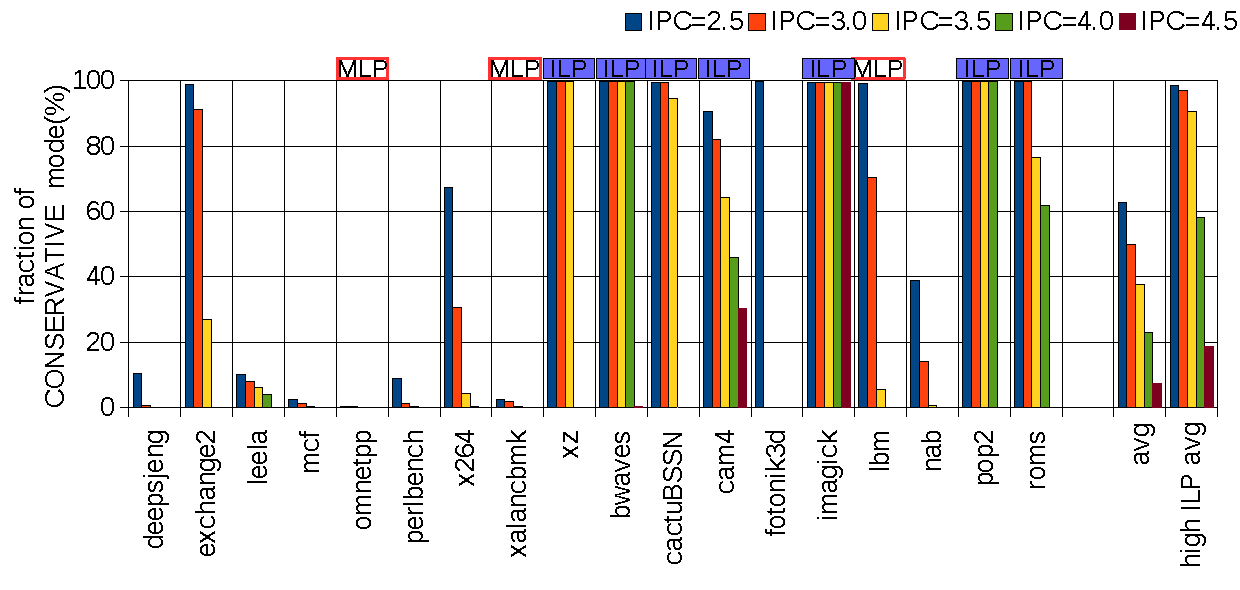
\includegraphics[keepaspectratio, scale=.8]{16_1_IPC}
  \caption{IPC を用いた SWITCH 方式の制御(16,1)}
  \label{fig:16_1_IPC}

  \centering
  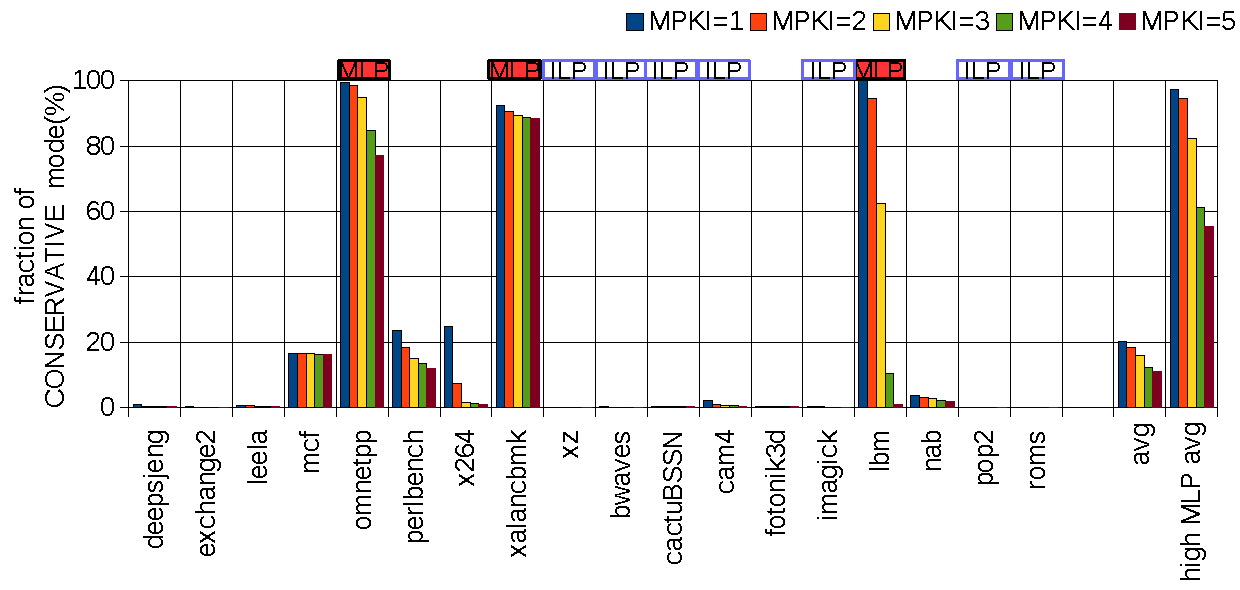
\includegraphics[keepaspectratio, scale=.8]{16_1_MPKI}
  \caption{LLC MPKI を用いた SWITCH 方式の制御(16,1)}
  \label{fig:16_1_MPKI}
\end{figure}

%(4,4)
\begin{figure}[tb]
  \centering
  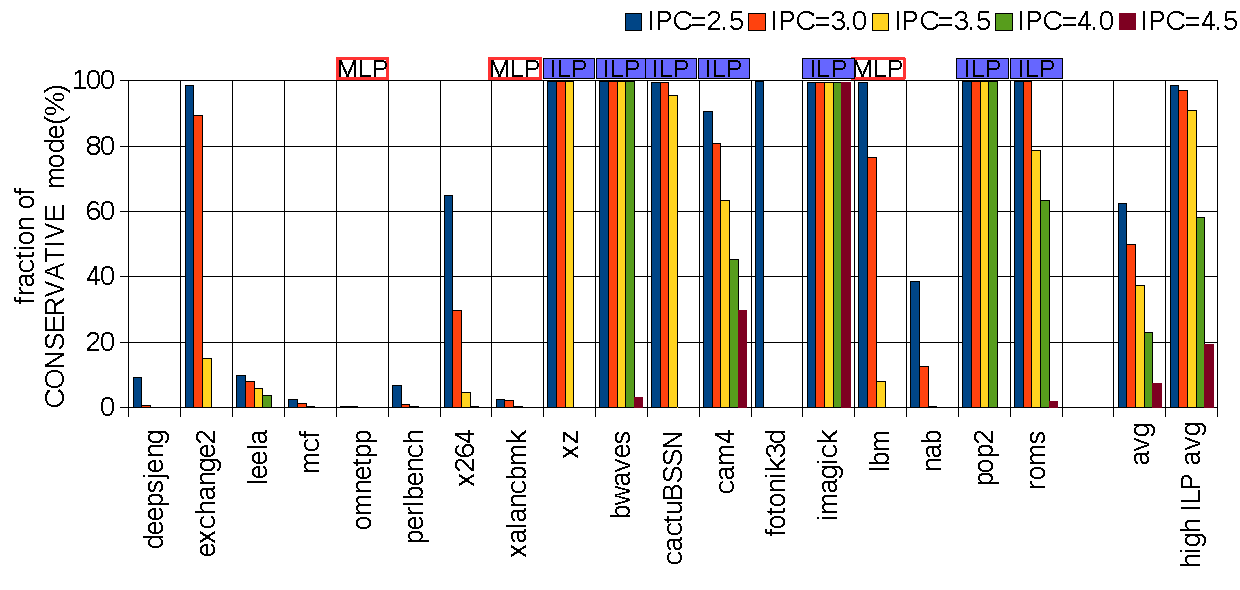
\includegraphics[keepaspectratio, scale=.8]{4_4_IPC}
  \caption{IPC を用いた SWITCH 方式の制御(4,4)}
  \label{fig:4_4_IPC}

  \centering
  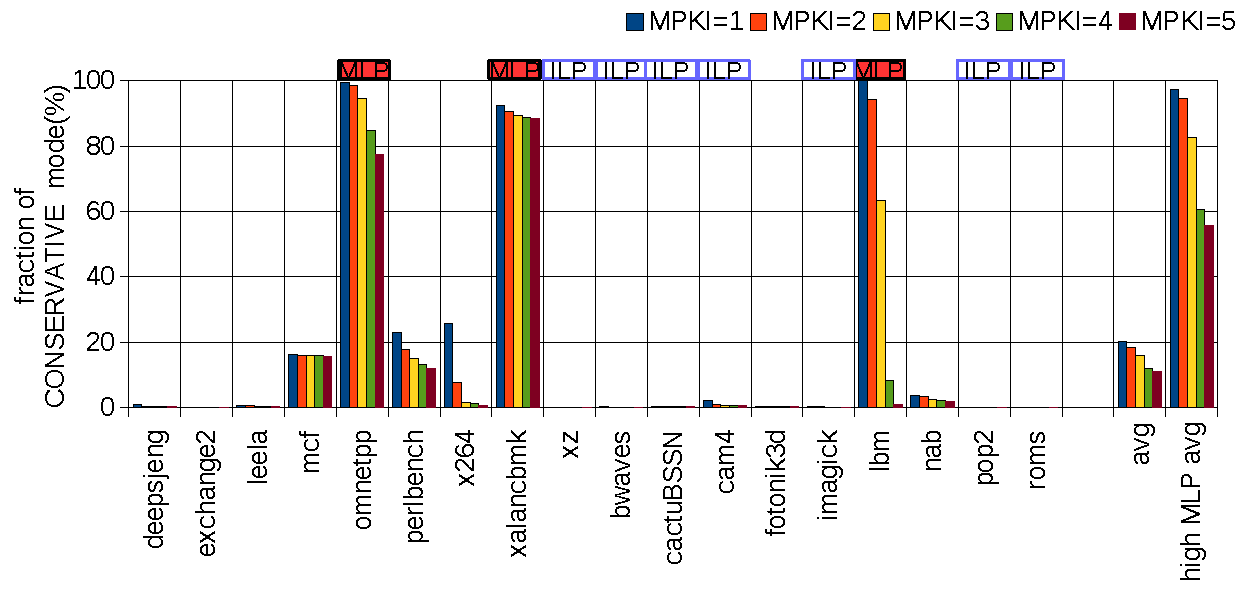
\includegraphics[keepaspectratio, scale=.8]{4_4_MPKI}
  \caption{LLC MPKI を用いた SWITCH 方式の制御(4,4)}
  \label{fig:4_4_MPKI}
\end{figure}

%(32,1)
\begin{figure}[tb]
  \centering
  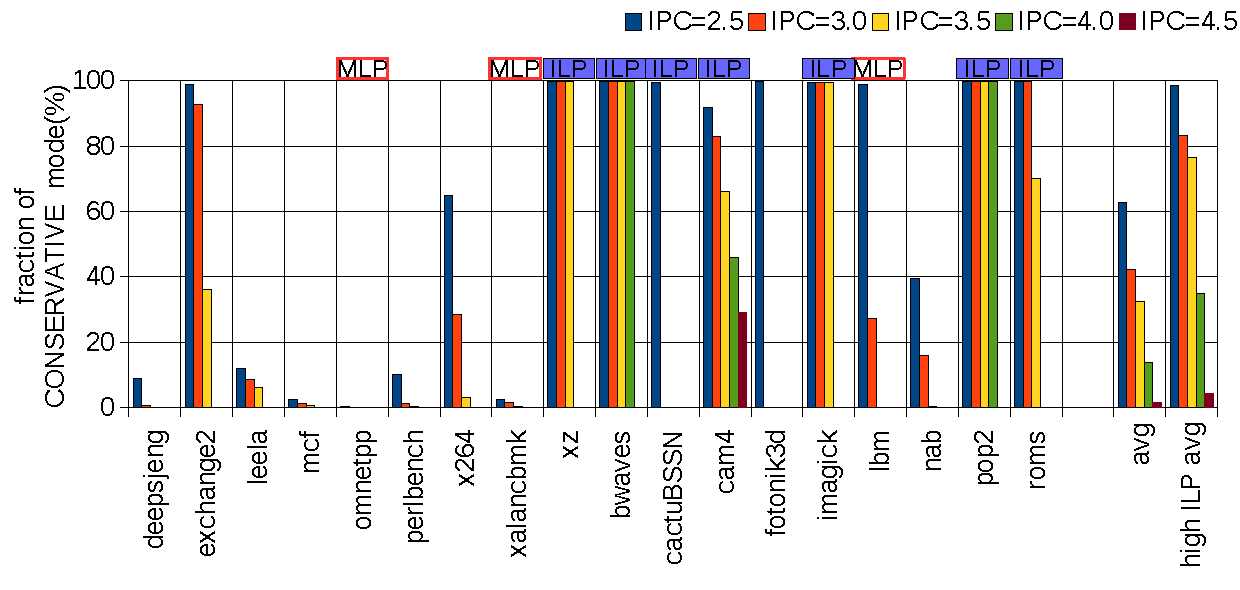
\includegraphics[keepaspectratio, scale=.8]{32_1_IPC}
  \caption{IPC を用いた SWITCH 方式の制御(32,1)}
  \label{fig:32_1_IPC}

  \centering
  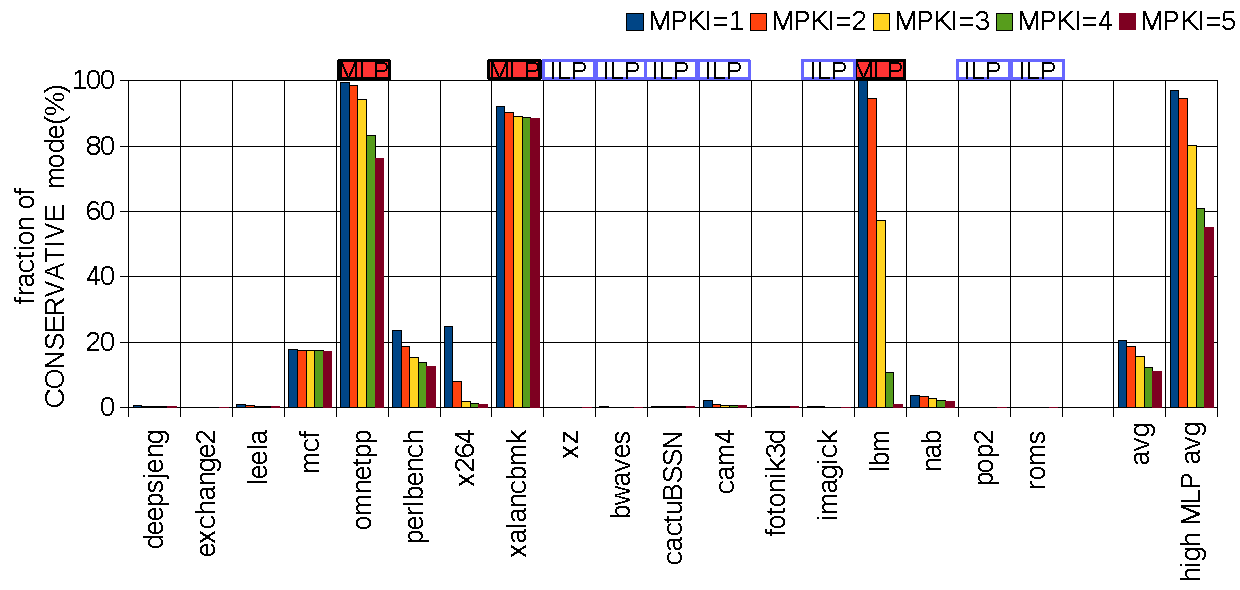
\includegraphics[keepaspectratio, scale=.8]{32_1_MPKI}
  \caption{LLC MPKI を用いた SWITCH 方式の制御(32,1)}
  \label{fig:32_1_MPKI}
\end{figure}

%(16,2)
\begin{figure}[tb]
  \centering
  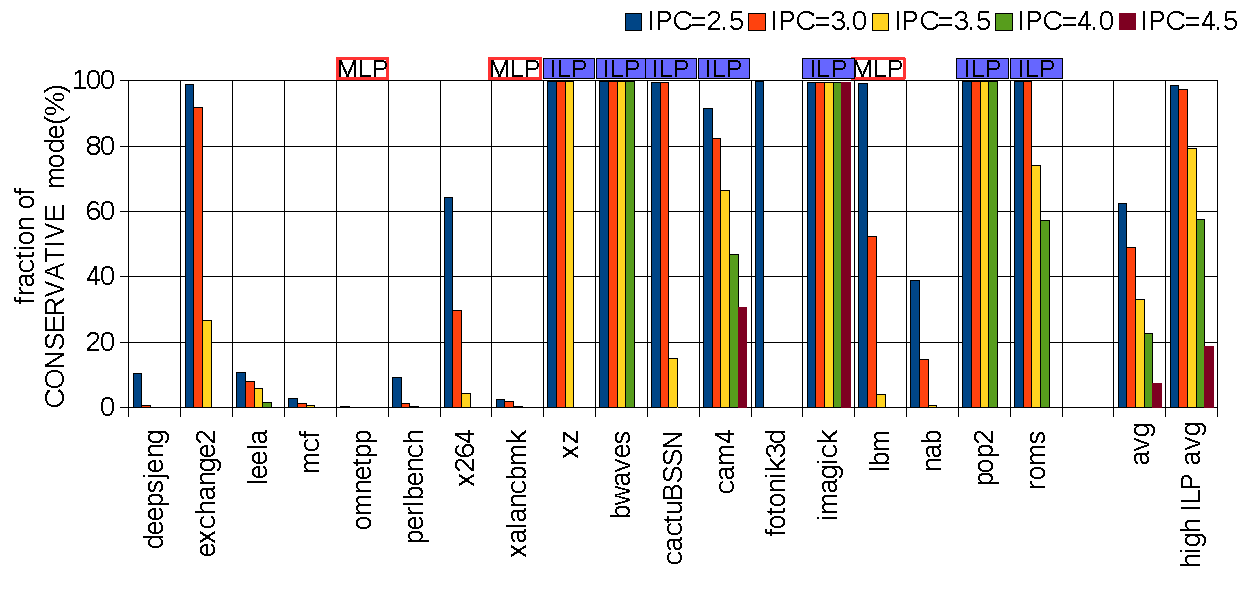
\includegraphics[keepaspectratio, scale=.8]{16_2_IPC}
  \caption{IPC を用いた SWITCH 方式の制御(16,2)}
  \label{fig:16_2_IPC}

  \centering
  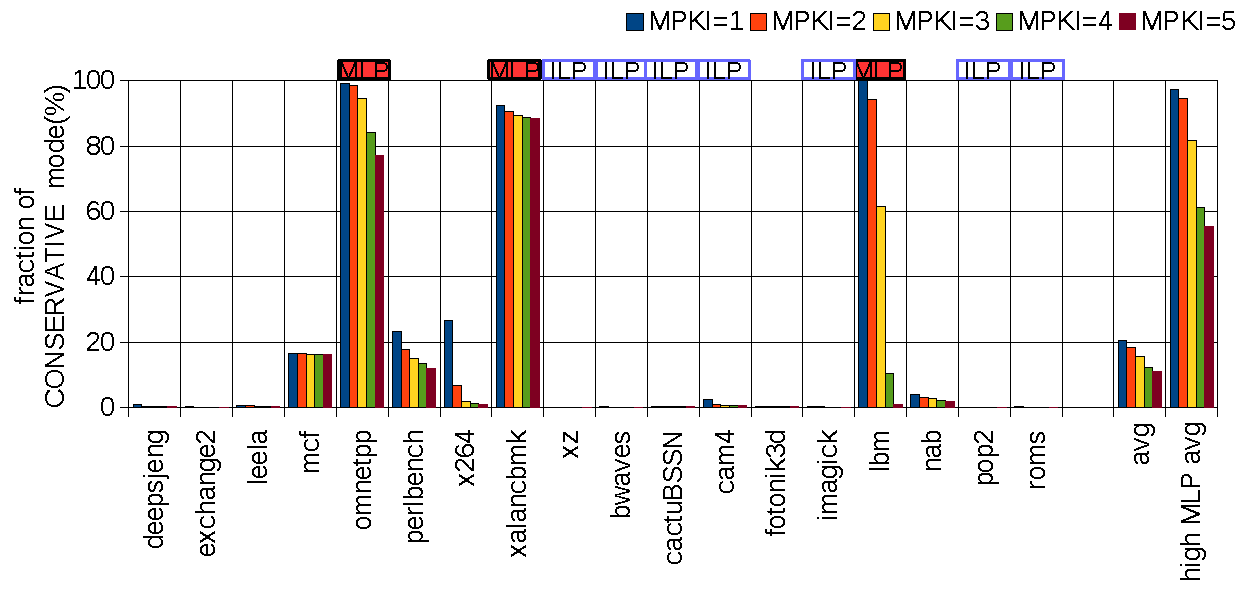
\includegraphics[keepaspectratio, scale=.8]{16_2_MPKI}
  \caption{LLC MPKI を用いた SWITCH 方式の制御(16,2)}
  \label{fig:16_2_MPKI}
\end{figure}

%(8,4)
\begin{figure}[tb]
  \centering
  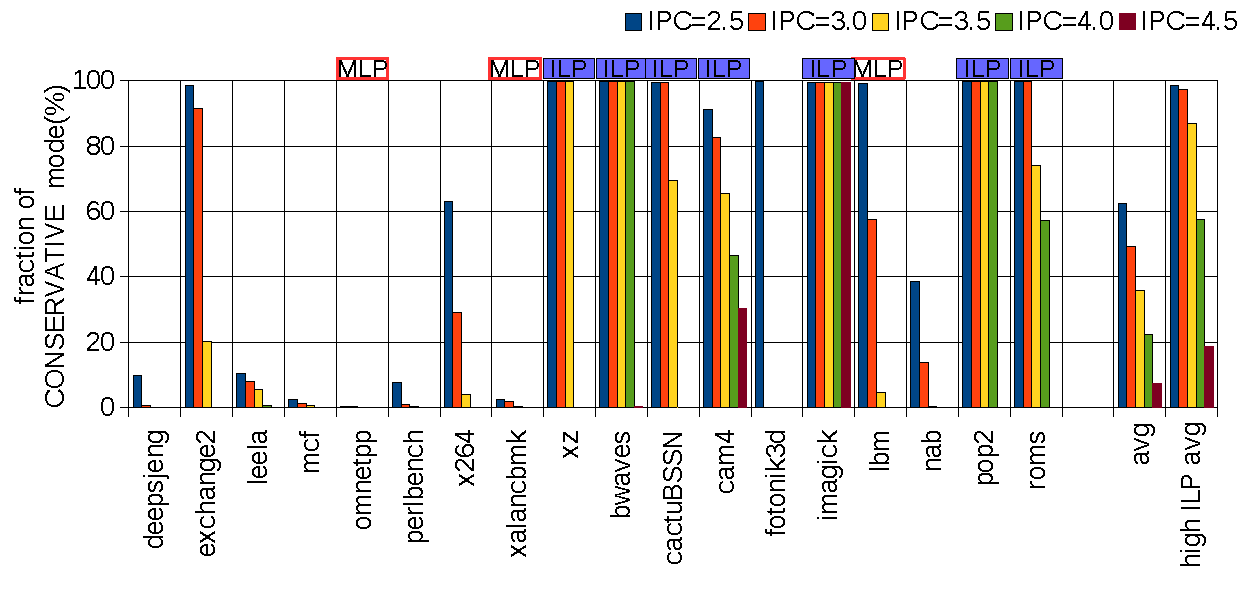
\includegraphics[keepaspectratio, scale=.8]{8_4_IPC}
  \caption{IPC を用いた SWITCH 方式の制御(8,4)}
  \label{fig:8_4_IPC}

  \centering
  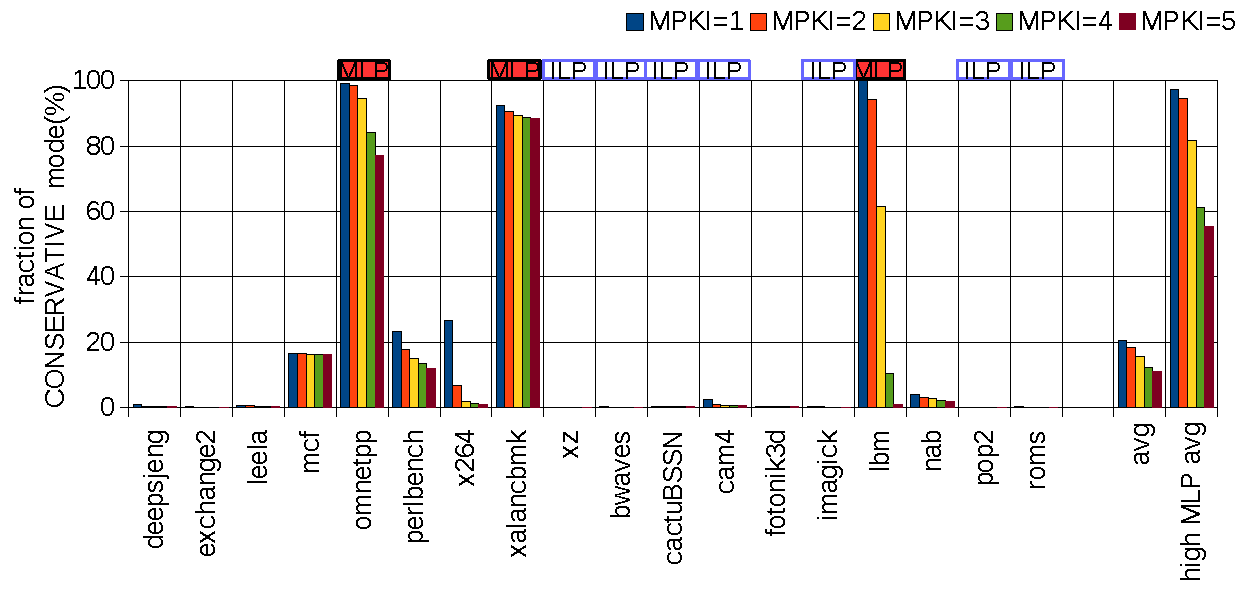
\includegraphics[keepaspectratio, scale=.8]{8_4_MPKI}
  \caption{LLC MPKI を用いた SWITCH 方式の制御(8,4)}
  \label{fig:8_4_MPKI}
\end{figure}
